\documentclass[12pt,a4paper]{article}
\usepackage[utf8]{vietnam}
\usepackage{amsmath,amssymb}
\usepackage{tabularx}
\usepackage{tikz}
\usetikzlibrary{calc,angles,quotes,arrows.meta,patterns}
\usepackage{xcolor}
\usepackage{enumitem}
\usepackage{fancyhdr}
\usepackage{graphicx}
\usepackage[top=0.9cm, bottom=0.9cm, left=1.2cm, right=1.2cm]{geometry}
\usepackage[loigiai]{ex_test}
\SAOPTN{widthSA=3.2,heightSA=0.62}

\setlength{\headheight}{15pt}
\setlength{\parskip}{0pt}

\pagestyle{fancy}
\fancyhf{}
\rhead{\textit{Môn Toán 8 -- Hướng dẫn giải Đề số 06}}
\lhead{\textit{Bộ đề ôn tập Giữa học kì I}}
\cfoot{\thepage}

\begin{document}

\begin{center}
  \textbf{\Large HƯỚNG DẪN GIẢI CHI TIẾT VÀ BẢNG ĐÁP ÁN}\\
  \textbf{\large ĐỀ ÔN TẬP GIỮA HỌC KỲ I -- ĐỀ SỐ 06}\\
  \textit{Môn: Toán 8 -- Năm học 2026 -- 2027}
\end{center}
\vspace{2mm}

% --- BẢNG ĐÁP ÁN TRẮC NGHIỆM TÓM TẮT ---
\noindent\textbf{\large A. BẢNG ĐÁP ÁN TRẮC NGHIỆM TỔNG HỢP}
\vspace{1mm}

\noindent\textbf{1. Phần I (Mỗi câu trả lời đúng được 0,25 điểm):}
\begin{center}
\begin{tabular}{|c|c|c|c|c|c|c|c|c|c|c|c|c|}
\hline
\textbf{Câu} & \textbf{1} & \textbf{2} & \textbf{3} & \textbf{4} & \textbf{5} & \textbf{6} & \textbf{7} & \textbf{8} & \textbf{9} & \textbf{10} & \textbf{11} & \textbf{12} \\
\hline
\textbf{Đ/A} & \textbf{A} & \textbf{C} & \textbf{B} & \textbf{B} & \textbf{A} & \textbf{A} & \textbf{D} & \textbf{A} & \textbf{C} & \textbf{C} & \textbf{C} & \textbf{C} \\
\hline
\end{tabular}
\end{center}
\vspace{0.5mm}

\noindent\textbf{2. Phần II (Đúng 1 ý: 0,1đ; 2 ý: 0,25đ; 3 ý: 0,5đ; 4 ý: 1,0đ):}
\begin{center}
\begin{tabular}{|c|c|c|c|c||c|c|c|c|c|}
\hline
\textbf{Câu} & \textbf{a)} & \textbf{b)} & \textbf{c)} & \textbf{d)} & \textbf{Câu} & \textbf{a)} & \textbf{b)} & \textbf{c)} & \textbf{d)} \\
\hline
\textbf{Câu 1} & \textbf{Đ} & \textbf{S} & \textbf{Đ} & \textbf{Đ} & \textbf{Câu 2} & \textbf{Đ} & \textbf{Đ} & \textbf{Đ} & \textbf{S} \\
\hline
\end{tabular}
\end{center}
\vspace{0.5mm}

\noindent\textbf{3. Phần III (Mỗi câu trả lời đúng được 1,0 điểm):}
\begin{center}
\begin{tabular}{|c|c|c|}
\hline
\textbf{Câu} & \textbf{Câu 1} & \textbf{Câu 2} \\
\hline
\textbf{Đáp án} & $\mathbf{x = 5 \text{ hoặc } x = \dfrac{1}{2}}$ & $\mathbf{10\text{ cm}}$ \\
\hline
\end{tabular}
\end{center}
\vspace{1.5mm}

% --- B. LỜI GIẢI CHI TIẾT ---
\noindent\textbf{\large B. LỜI GIẢI CHI TIẾT CÁC CÂU HỎI}
\vspace{1mm}
\begin{ex}
Đơn thức $-36a^2b^2x^2y^2$ (với $a, b$ là các hằng số) có hệ số là:
\choice
{\True $-36a^2b^2$}
{$-36$}
{$36a^2b^2$}
{$36a^2$}
\loigiai{
Hệ số của đơn thức bao gồm toàn bộ phần hằng số đứng trước các biến, do đó hệ số là $-36a^2b^2$.
}
\end{ex}

\begin{ex}
Đơn thức nào sau đây đồng dạng với đơn thức $-3x^2y$?
\choice
{$3x^2yz$}
{$xy^2$}
{\True $\dfrac{1}{2}xyx$}
{$-3x^2z$}
\loigiai{
Rút gọn đơn thức ở phương án C: $\dfrac{1}{2}xyx = \dfrac{1}{2}x^2y$, đơn thức này có cùng phần biến $x^2y$ với đơn thức $-3x^2y$.
}
\end{ex}

\begin{ex}
Tích của đơn thức $6xy$ và đa thức $2x^2 - 3y$ là đa thức:
\choice
{$12x^3y + 18xy^2$}
{\True $12x^3y - 18xy^2$}
{$12x^2y + 18xy^2$}
{$12x^2y - 18xy^2$}
\loigiai{
Thực hiện phép nhân: $6xy \cdot (2x^2 - 3y) = 6xy \cdot 2x^2 - 6xy \cdot 3y = 12x^3y - 18xy^2$.
}
\end{ex}

\begin{ex}
Điều kiện của số tự nhiên $n$ để phép chia $(4x^{10}y - xy^7 + x^5y^4) : 2x^n y^n$ là phép chia hết:
\choice
{$n = 0$}
{\True $n \in \{0; 1\}$}
{$n = 1$}
{$n = 5$}
\loigiai{
Đa thức chia hết cho đơn thức khi số mũ của mỗi biến trong đơn thức chia nhỏ hơn hoặc bằng số mũ nhỏ nhất của biến đó trong các hạng tử của đa thức. Số mũ nhỏ nhất của $x$ và $y$ trong đa thức là $1$, do đó $n \le 1$. Vì $n$ là số tự nhiên nên $n \in \{0; 1\}$.
}
\end{ex}

\begin{ex}
Hình bình hành cần có thêm điều kiện nào sau đây thì trở thành hình chữ nhật?
\choice
{\True Có một góc vuông}
{Có hai cạnh kề bằng nhau}
{Có hai đường chéo vuông góc}
{Có hai đường chéo cắt nhau tại trung điểm mỗi đường}
\loigiai{
Theo dấu hiệu nhận biết, hình bình hành có một góc vuông là hình chữ nhật.
}
\end{ex}

\begin{ex}
Tích của hai đơn thức $7x^2y$ và $(-xy)$ bằng:
\choice
{\True $-7x^3y^2$}
{$7x^3y^2$}
{$-7x^2y$}
{$6x^3y^2$}
\loigiai{
Ta có: $7x^2y \cdot (-xy) = 7 \cdot (-1) \cdot (x^2 \cdot x) \cdot (y \cdot y) = -7x^3y^2$.
}
\end{ex}

\begin{ex}
Kết quả thu gọn của biểu thức $(x + 3)^2 - (x - 3)^2$ là:
\choice
{$0$}
{$18$}
{$12x + 18$}
{\True $12x$}
\loigiai{
Áp dụng hằng đẳng thức hiệu hai bình phương: $(x + 3)^2 - (x - 3)^2 = [(x + 3) - (x - 3)][(x + 3) + (x - 3)] = 6 \cdot 2x = 12x$.
}
\end{ex}

\begin{ex}
Cho hình vẽ sau, trung đoạn của hình chóp tứ giác đều $S.ABCD$ là đoạn thẳng:
\begin{center}
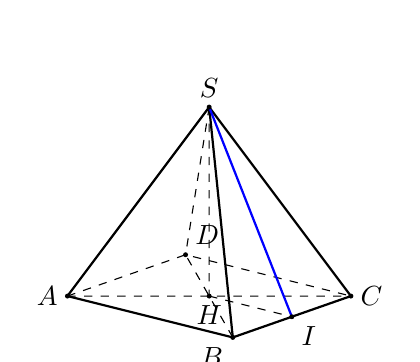
\begin{tikzpicture}[scale=0.75, >=stealth]
  \coordinate (A) at (0,0);
  \coordinate (B) at (2.8,-0.7);
  \coordinate (C) at (4.8,0);
  \coordinate (D) at (2,0.7);
  \coordinate (H) at ($(A)!0.5!(C)$);
  \coordinate (S) at ($(H)+(0,3.2)$);
  \coordinate (I) at ($(B)!0.5!(C)$);
  \draw[dashed] (A)--(D)--(C);
  \draw[dashed] (S)--(D);
  \draw[dashed] (A)--(C) (B)--(D);
  \draw[dashed] (S)--(H);
  \draw[dashed] (H)--(I);
  \draw[thick] (S)--(A)--(B)--(C)--(S);
  \draw[thick] (S)--(B);
  \draw[thick, blue] (S)--(I);
  \fill (A) circle (1.2pt) node[left] {$A$};
  \fill (B) circle (1.2pt) node[below left] {$B$};
  \fill (C) circle (1.2pt) node[right] {$C$};
  \fill (D) circle (1.2pt) node[above right] {$D$};
  \fill (S) circle (1.2pt) node[above] {$S$};
  \fill (H) circle (1.2pt) node[below] {$H$};
  \fill (I) circle (1.2pt) node[below right] {$I$};
\end{tikzpicture}
\end{center}
\choice
{\True $SI$}
{$SA$}
{$SH$}
{$HI$}
\loigiai{
Trung đoạn của hình chóp tứ giác đều là đường cao của mặt bên xuất phát từ đỉnh hình chóp. Trong hình, đoạn thẳng $SI$ là đường cao của mặt bên tam giác $SBC$.
}
\end{ex}

\begin{ex}
Hình chóp tứ giác đều có mặt đáy là hình gì?
\choice
{Tam giác đều}
{Hình chữ nhật}
{\True Hình vuông}
{Hình thoi}
\loigiai{
Theo định nghĩa, hình chóp tứ giác đều có mặt đáy là hình vuông.
}
\end{ex}

\begin{ex}
Tứ giác là hình bình hành nếu:
\choice
{Tứ giác có hai góc kề một cạnh bằng nhau}
{Tứ giác có hai cạnh kề bằng nhau}
{\True Tứ giác có các cạnh đối bằng nhau}
{Tứ giác có hai đường chéo bằng nhau}
\loigiai{
Dấu hiệu nhận biết hình bình hành: tứ giác có các cạnh đối bằng nhau là hình bình hành.
}
\end{ex}

\begin{ex}
Khẳng định nào sau đây là đúng?
\choice
{Tứ giác có hai đường chéo vuông góc với nhau là hình bình hành}
{Tứ giác có hai đường chéo bằng nhau là hình thang cân}
{\True Tứ giác có hai đường chéo cắt nhau tại trung điểm mỗi đường là hình bình hành}
{Hình thang có hai cạnh bằng nhau là hình thang cân}
\loigiai{
Theo dấu hiệu nhận biết, tứ giác có hai đường chéo cắt nhau tại trung điểm của mỗi đường là hình bình hành.
}
\end{ex}

\begin{ex}
Cho tam giác $ABC$ vuông tại $A$ có $AB = 6\text{ cm}, AC = 8\text{ cm}$. Bán kính đường tròn ngoại tiếp tam giác $ABC$ bằng:
\choice
{$10\text{ cm}$}
{$14\text{ cm}$}
{\True $5\text{ cm}$}
{$7\text{ cm}$}
\loigiai{
Cạnh huyền $BC = \sqrt{AB^2 + AC^2} = \sqrt{6^2 + 8^2} = 10\text{ cm}$. Tâm đường tròn ngoại tiếp tam giác vuông là trung điểm cạnh huyền, bán kính $R = \dfrac{BC}{2} = 5\text{ cm}$.
}
\end{ex}


\setcounter{ex}{0}
\noindent\textbf{\large PHẦN II. CÂU TRẮC NGHIỆM ĐÚNG SAI}
\vspace{1mm}
\begin{ex}
Cho biểu thức $A = \dfrac{x^2 - 4x + 4}{x - 2} + \dfrac{x^2 - 9}{x + 3}$ với $x \neq 2$ và $x \neq -3$. Xét tính đúng sai của các mệnh đề sau:
\choiceTF
{\True Biến đổi $x^2 - 4x + 4$ thành bình phương của một hiệu ta được $(x - 2)^2$}
{Kết quả rút gọn phân thức $\dfrac{x^2 - 9}{x + 3}$ là $x + 3$}
{\True Kết quả rút gọn của biểu thức $A$ là $2x - 5$}
{\True Tại $x = 4$, giá trị của biểu thức $A$ bằng $3$}
\loigiai{
\textbf{a)} \textbf{Đúng.} Áp dụng hằng đẳng thức: $x^2 - 4x + 4 = (x - 2)^2$.

\textbf{b)} \textbf{Sai.} Ta có $\dfrac{x^2 - 9}{x + 3} = \dfrac{(x - 3)(x + 3)}{x + 3} = x - 3$.

\textbf{c)} \textbf{Đúng.} $A = \dfrac{(x - 2)^2}{x - 2} + \dfrac{(x - 3)(x + 3)}{x + 3} = (x - 2) + (x - 3) = 2x - 5$.

\textbf{d)} \textbf{Đúng.} Thay $x = 4$ vào biểu thức rút gọn: $A = 2 \cdot 4 - 5 = 3$.
}
\end{ex}

\begin{ex}
Cho hình bình hành $ABCD$ có $AB = 2AD$. Gọi $M, N$ lần lượt là trung điểm của $AB$ và $CD$. Xét tính đúng sai của các mệnh đề sau:
\choiceTF
{\True Tứ giác $AMCN$ là hình bình hành}
{\True Tứ giác $AMND$ là hình thoi}
{\True Đoạn thẳng $AN$ vuông góc với đoạn thẳng $DM$}
{Cho $\widehat{A} = 60^\circ$, số đo góc $\widehat{AMD}$ bằng $120^\circ$}
\loigiai{
\textbf{a)} \textbf{Đúng.} Ta có $AM \parallel NC$ và $AM = NC = \dfrac{1}{2}AB$, do đó $AMCN$ là hình bình hành.

\textbf{b)} \textbf{Đúng.} Tứ giác $AMND$ có $AM \parallel DN$ và $AM = DN = AD$ nên là hình bình hành có hai cạnh kề bằng nhau, do đó $AMND$ là hình thoi.

\textbf{c)} \textbf{Đúng.} $AN$ và $DM$ là hai đường chéo của hình thoi $AMND$ nên $AN \perp DM$.

\textbf{d)} \textbf{Sai.} Tam giác $AMD$ có $AM = AD$ và $\widehat{A} = 60^\circ$ nên là tam giác đều, do đó $\widehat{AMD} = 60^\circ$.
}
\end{ex}


\setcounter{ex}{0}
\noindent\textbf{\large PHẦN III. CÂU HỎI TRẢ LỜI NGẮN}
\vspace{1mm}
\begin{ex}
Tìm $x$, biết: $2x(x - 5) - x + 5 = 0$. \shortans{$x = 5$ hoặc $x = \dfrac{1}{2}$}
\loigiai{
Ta có: $2x(x - 5) - (x - 5) = 0 \Leftrightarrow (x - 5)(2x - 1) = 0$.

- Trường hợp 1: $x - 5 = 0 \Leftrightarrow x = 5$.

- Trường hợp 2: $2x - 1 = 0 \Leftrightarrow x = \dfrac{1}{2}$.

Vậy $x = 5$ hoặc $x = \dfrac{1}{2}$.
}
\end{ex}

\begin{ex}
Cho hình chữ nhật $ABCD$ có $AB = 8\text{ cm}$ và $BC = 6\text{ cm}$. Tính độ dài đường chéo $AC$. \shortans{$10\text{ cm}$}
\loigiai{
Áp dụng định lý Pythagore trong tam giác vuông $ABC$ vuông tại $B$:

$AC^2 = AB^2 + BC^2 = 8^2 + 6^2 = 64 + 36 = 100$.

Suy ra $AC = \sqrt{100} = 10\text{ cm}$.
}
\end{ex}


\setcounter{ex}{0}
\noindent\textbf{\large PHẦN IV. TỰ LUẬN (HƯỚNG DẪN GIẢI VÀ THANG ĐIỂM)}
\vspace{1mm}
\begin{ex} (1,0 điểm)
Thực hiện phép tính:
\begin{enumerate}[label=\textbf{\alph*)}, leftmargin=0.8cm, itemsep=0pt, topsep=1pt]
\item (0,5 điểm) $xy(x^2 - 5xy^2)$
\item (0,5 điểm) $(12x^4y^3 - 5x^3y^2 + 9x^2y^2) : (-3x^2y^2)$
\end{enumerate}
\loigiai{
\textbf{a)} \textit (0,5 điểm): $xy(x^2 - 5xy^2) = xy \cdot x^2 - xy \cdot 5xy^2 = x^3y - 5x^2y^3$.

\textbf{b)} \textit (0,5 điểm): $(12x^4y^3 - 5x^3y^2 + 9x^2y^2) : (-3x^2y^2) = 12x^4y^3 : (-3x^2y^2) - 5x^3y^2 : (-3x^2y^2) + 9x^2y^2 : (-3x^2y^2) = -4x^2y + \dfrac{5}{3}x - 3$.


}
\end{ex}
\vspace{0.5mm}

\begin{ex} (0,75 điểm)
Cho hai đa thức: $M = xy - 3x^2y^2 + x^4 - 5y^3$ và $N = x^4 - 5y^3 - 2x^2y^2 - xy$.
\begin{enumerate}[label=\textbf{\alph*)}, leftmargin=0.8cm, itemsep=0pt, topsep=1pt]
\item (0,4 điểm) Tìm đa thức $P = M - N$.
\item (0,35 điểm) Tính giá trị của đa thức $P$ tại $x = -1, y = -1$.
\end{enumerate}
\loigiai{
\textbf{a)} \textit (0,4 điểm): $P = (xy - 3x^2y^2 + x^4 - 5y^3) - (x^4 - 5y^3 - 2x^2y^2 - xy) = (x^4 - x^4) + (-5y^3 + 5y^3) + (-3x^2y^2 + 2x^2y^2) + (xy + xy) = -x^2y^2 + 2xy$.

\textbf{b)} \textit (0,35 điểm): Thay $x = -1, y = -1$ vào $P$: $P = -(-1)^2 \cdot (-1)^2 + 2(-1)(-1) = -(1 \cdot 1) + 2 = -1 + 2 = 1$.


}
\end{ex}
\vspace{0.5mm}

\begin{ex} (0,75 điểm)
Tháp tài chính Bitexco có 68 tầng (không kể các tầng hầm). Biết rằng khi tòa tháp có bóng $MP$ in trên mặt đất dài $47{,}5\text{ m}$ thì cùng thời điểm đó có một cột cờ $AB$ cao $12\text{ m}$ có bóng $AP$ in trên mặt đất dài $2{,}12\text{ m}$ (như hình vẽ). Tính chiều cao $MN$ của tháp tài chính Bitexco theo đơn vị mét (làm tròn kết quả đến hàng đơn vị).
\begin{center}
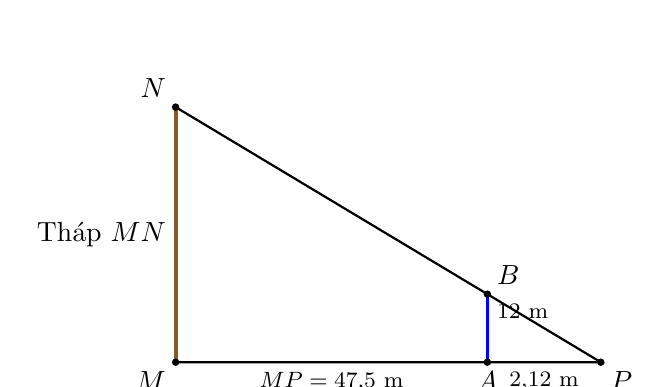
\begin{tikzpicture}[scale=0.9, >=stealth]
  \coordinate (M) at (0,0);
  \coordinate (N) at (0,3.6);
  \coordinate (P) at (6,0);
  \coordinate (A) at (4.4,0);
  \coordinate (B) at (4.4,0.96);
  \draw[thick] (M)--(P)--(N)--cycle;
  \draw[thick, blue] (A)--(B);
  \draw[line width=1.5pt, brown!70!black] (M)--(N);
  \fill (M) circle (1.5pt) node[below left] {$M$};
  \fill (N) circle (1.5pt) node[above left] {$N$};
  \fill (P) circle (1.5pt) node[below right] {$P$};
  \fill (A) circle (1.5pt) node[below] {$A$};
  \fill (B) circle (1.5pt) node[above right] {$B$};
  \node[left] at ($(M)!0.5!(N)$) {Tháp $MN$};
  \node[above right] at ($(A)!0.5!(B)$) {\footnotesize $12\text{ m}$};
  \node[below] at ($(A)!0.5!(P)$) {\footnotesize $2{,}12\text{ m}$};
  \node[below] at ($(M)!0.5!(A)$) {\footnotesize $MP = 47{,}5\text{ m}$};
\end{tikzpicture}
\end{center}
\begin{enumerate}[label=\textbf{\alph*)}, leftmargin=0.8cm, itemsep=0pt, topsep=1pt]
\item (0,75 điểm) Tính chiều cao $MN$ của tháp Bitexco.
\end{enumerate}
\loigiai{
\textbf{a)} \textit (0,75 điểm): Tòa tháp Bitexco $MN$ và cột cờ $AB$ đều dựng vuông góc với mặt đất $MP$, do đó $AB \parallel MN$.

Xét tam giác $NMP$ có $AB \parallel MN$, theo định lý Ta-lét ta có: $\dfrac{AB}{MN} = \dfrac{AP}{MP}$.

Thay số: $\dfrac{12}{MN} = \dfrac{2{,}12}{47{,}5} \Rightarrow MN = \dfrac{12 \cdot 47{,}5}{2{,}12} = \dfrac{570}{2{,}12} \approx 268{,}87\text{ m}$.

Làm tròn đến hàng đơn vị, chiều cao của tháp xấp xỉ $269\text{ m}$.


}
\end{ex}
\vspace{0.5mm}

\begin{ex} (0,5 điểm)
Chứng minh rằng $A = x^2 + 2xy + 4y^2 + 6y + 5 > 0$ với mọi $x, y$.
\begin{enumerate}[label=\textbf{\alph*)}, leftmargin=0.8cm, itemsep=0pt, topsep=1pt]
\item (0,5 điểm) Chứng minh $A > 0$ với mọi $x, y$.
\end{enumerate}
\loigiai{
\textbf{a)} \textit (0,5 điểm): Ta biến đổi biểu thức $A$ như sau:

$A = (x^2 + 2xy + y^2) + (3y^2 + 6y + 3) + 2$

$= (x + y)^2 + 3(y^2 + 2y + 1) + 2$

$= (x + y)^2 + 3(y + 1)^2 + 2$.

Vì $(x + y)^2 \ge 0$ và $3(y + 1)^2 \ge 0$ với mọi $x, y$, nên $(x + y)^2 + 3(y + 1)^2 + 2 \ge 2 > 0$ với mọi $x, y$.

Vậy $A > 0$ với mọi $x, y$.


}
\end{ex}
\vspace{0.5mm}


\enlargethispage{1.5cm}
\begin{center}
\rule{4cm}{0.4pt}\\
\textit{--- HẾT ---}
\end{center}
\end{document}
